\documentclass{article}

% if you need to pass options to natbib, use, e.g.:
%     \PassOptionsToPackage{numbers, compress}{natbib}
% before loading neurips_2025

% The authors should use one of these tracks.
% Before accepting by the NeurIPS conference, select one of the options below.
% 0. "default" for submission
 % \usepackage{neurips_2025}
% the "default" option is equal to the "main" option, which is used for the Main Track with double-blind reviewing.
% 1. "main" option is used for the Main Track
%  \usepackage[main]{neurips_2025}
% 2. "position" option is used for the Position Paper Track
%  \usepackage[position]{neurips_2025}
% 3. "dandb" option is used for the Datasets & Benchmarks Track
 % \usepackage[dandb]{neurips_2025}
% 4. "creativeai" option is used for the Creative AI Track
%  \usepackage[creativeai]{neurips_2025}
% 5. "sglblindworkshop" option is used for the Workshop with single-blind reviewing
 % \usepackage[sglblindworkshop]{neurips_2025}
% 6. "dblblindworkshop" option is used for the Workshop with double-blind reviewing
%  \usepackage[dblblindworkshop]{neurips_2025}

% After being accepted, the authors should add "final" behind the track to compile a camera-ready version.
% 1. Main Track
 % \usepackage[main, final]{neurips_2025}
% 2. Position Paper Track
%  \usepackage[position, final]{neurips_2025}
% 3. Datasets & Benchmarks Track
 % \usepackage[dandb, final]{neurips_2025}
% 4. Creative AI Track
%  \usepackage[creativeai, final]{neurips_2025}
% 5. Workshop with single-blind reviewing
%  \usepackage[sglblindworkshop, final]{neurips_2025}
% 6. Workshop with double-blind reviewing
%  \usepackage[dblblindworkshop, final]{neurips_2025}
% Note. For the workshop paper template, both \title{} and \workshoptitle{} are required, with the former indicating the paper title shown in the title and the latter indicating the workshop title displayed in the footnote.
% For workshops (5., 6.), the authors should add the name of the workshop, "\workshoptitle" command is used to set the workshop title.
% \workshoptitle{WORKSHOP TITLE}

% "preprint" option is used for arXiv or other preprint submissions
 % \usepackage[preprint]{neurips_2025}

% to avoid loading the natbib package, add option nonatbib:
%    \usepackage[nonatbib]{neurips_2025}

% if you need to pass options to natbib, use, e.g.:
%     \PassOptionsToPackage{numbers, compress}{natbib}
% before loading neurips_data_2024

\usepackage[preprint]{neurips_2025}

% to compile a preprint version, add the [preprint] option, e.g.:
%     \usepackage[preprint]{neurips_data_2024}
% This will indicate that the work is currently under review.

% to compile a camera-ready version, add the [final] option, e.g.:
%     \usepackage[final]{neurips_data_2024}

% to avoid loading the natbib package, add option nonatbib:
%    \usepackage[nonatbib]{neurips_data_2024}

% Submissions to the datasets and benchmarks are typically non anonymous,
% but anonymous submissions are allowed. If you feel that you must submit 
% anonymously, you can compile an anonymous version by adding the [anonymous] 
% option, e.g.:
%     \usepackage[anonymous]{neurips_data_2024}
% This will hide all author names.


%% WARNING!
% To compile for arxiv, follow the instructions at 
% https://tex.stackexchange.com/questions/280590/work-around-for-minted-code-highlighting-in-arxiv#comment1207889_414781
%% ENDWARDNING

% - Imports
\usepackage[utf8]{inputenc} % allow utf-8 input
\usepackage[T1]{fontenc}    % use 8-bit T1 fonts
\usepackage{hyperref}       % hyperlinks
\usepackage{nicefrac}       % compact symbols for 1/2, etc.
\usepackage{microtype}      % microtypography
\usepackage{rotating}
\usepackage{graphicx}
\usepackage{nameref}
\usepackage{subcaption}
\usepackage{amsmath,amsthm,trimclip}
\usepackage{amssymb}
\usepackage{amsfonts}
\usepackage{footnote}
\usepackage{url}
\usepackage{lipsum}
\usepackage[acronym]{glossaries}
\usepackage{bbm}
\usepackage{adjustbox}
\usepackage{algorithm} 
\usepackage{algpseudocode}
\usepackage{booktabs}
\usepackage{mdframed}
\usepackage{color, colortbl}
\usepackage{xcolor}
\usepackage{placeins}
\usepackage{capt-of}
\usepackage{float}
\usepackage{newfloat}

\usepackage{enumitem}
\newlist{enumerate*}{enumerate}{1}
\setlist[enumerate*]{label=\arabic*, itemjoin={{, }}, itemjoin*={{, and }}, before*={}, after*={}}

\PassOptionsToPackage{table}{xcolor}

\definecolor{gemma}{HTML}{1B98E0}
\definecolor{llama}{HTML}{76C7C0}
\definecolor{mistral}{HTML}{FFD79D}
\definecolor{commandr}{HTML}{02475E}

% Operators
\newcommand{\ent}[0]{\mathcal{H}}
\newcommand{\cred}[0]{c}
\newcommand{\info}[0]{\mathcal{I}_z}
\newcommand{\E}[0]{\mathop{\mathbb{E}}}
\newcommand{\prob}[0]{\mathbb{P}}
\newcommand{\wip}[0]{\textcolor{orange}{[WIP] }}
\newcommand{\argmax}{\mathop{\mathrm{argmax}}}
\newcommand{\argsup}{\mathop{\mathrm{argsup}}}
\newcommand{\argmin}{\mathop{\mathrm{argmin}}}
\newcommand{\arginf}{\mathop{\mathrm{arginf}}}
\newcommand{\supp}{\mathop{\mathrm{supp}}}

% Theorems and definitions
\newtheorem{definition}{Definition}
\newtheorem{property}{Property}
\newtheoremstyle{postulate}{1em}{1em}{}{}{\bfseries}{\normalfont\textit{.}}{.5em}{}
\theoremstyle{postulate}
\newtheorem{postulate}{Postulate}

% Floats
\floatstyle{plain}
\newfloat{snippet}{H}{lop}
\floatname{snippet}{Code}


% Enter the title of your paper:
\title{Latent option models: discovering temporally-extended actions from actionless data}

% The "running title" will be displayed in the header on every-other page.
% It is typically either the same as the title or a shorter version of the title.
% Enter your running title here:

% WARNING: Authors must not appear in the submitted version. They should be hidden
% as long as the rlj package is used without the [accepted] or [preprint] options.
% Non-anonymous submissions will be rejected without review.

% Enter the author names below. 
% NOTE: Denote affiliations using superscripts as in the provided example.
% NOTE: Use \textscript{1,2,3} instead of $^{1,2,3}$.
%       - Failure to do so will cause affiliation superscripts to appear on the cover page for camera-ready and preprint versions.
\author{%
Eduardo Pignatelli \\
University College London \\
\texttt{e.pignatelli@ucl.ac.uk}
}
% ---------------------------------------------------------------------------





% ---------------------------------------------------------------------------
% - Document start  ---------------------------------------------------------
% ---------------------------------------------------------------------------
\begin{document}

\maketitle


% - Acronyms
\glsdisablehyper  % disables hyperlink to acronyms

\newacronym{rl}{RL}{Reinforcement Learning}
\newacronym{drl}{Deep RL}{Deep Reinforcement Learning}
\newacronym[longplural=Random Processes]{rp}{RP}{Random Process}
\newacronym[longplural=Markov Processes]{mp}{MP}{Markov Process}
\newacronym[longplural=Markov Reward Processes]{mrp}{MRP}{Markov Reward Process}
\newacronym[longplural=Markov Decision Processes]{mdp}{MDP}{Markov Decision Process}
\newacronym[longplural=Partially-observable Markov Decision Processes]{pomdp}{POMDP}{Partially-observable Markov Decision Process}
\newacronym{ca}{CA}{Credit Assignment}
\newacronym{cap}{CAP}{Credit Assignment Problem}
\newacronym{hi}{HI}{Hindsight Information}
\newacronym{gpi}{GPI}{Generalised Policy Iteration}
\newacronym{mpi}{MPI}{Modified Policy Iteration}
\newacronym{pe}{PE}{Policy Evaluation}
\newacronym{pi}{PI}{Policy Improvement}
\newacronym{lstm}{LSTM}{Long-Short-Term-Memory}
\newacronym{td}{TD}{Temporal Difference}
\newacronym{kl}{KL}{Kullback-Leibler}
\newacronym{dnn}{DNN}{Deep Neural Network}
\newacronym{llm}{LLM}{Large Language Model}
\newacronym{vlm}{VLM}{Vision Language Model}
\newacronym{calm}{CALM}{Credit Assignment with Language Models}
\newacronym{hrl}{HRL}{Hierarchical Reinforcement Learning}
\newacronym{xla}{XLA}{Accelerated Linear Algebra}
\newacronym{ecsm}{ECSM}{Entity-Component-System Model}
\newacronym{lom}{LOM}{Latent Option Model}
\newacronym{lam}{LAM}{Latent Action Model}
\newacronym{sol}{SOL}{Scalable Option Learning}
\newacronym{genie}{GENIE}{Generative Interaction Environment}
% ---


% ---------------------------------------------------------------------------
% - Abstract   --------------------------------------------------------------
% ---------------------------------------------------------------------------
\begin{abstract}

\end{abstract}

% ---------------------------------------------------------------------------
% - Introduction  -----------------------------------------------------------
% ---------------------------------------------------------------------------
\section{Introduction}
\label{sec:introduction}

\begin{figure}[!b]
    \centering
    \includegraphics[width=0.9\textwidth, height=0.4\textwidth]{example-image.png}
    \caption{Average episodic return of a \gls{lom} agent compared to flat and hierarchical baselines on a long-horizon task.}
    \label{fig:lom-results}
\end{figure}

% RL importance
The last few years have consolidated the importance of \gls{rl} in developing agents that can solve general tasks.
Agents trained with \gls{rl} can now align the behaviour of frontier language models~\citep{ouyang2022instructgpt}, unlock emergent reasoning capabilities without human-labelled demonstrations~\citep{deepseekr1}, predict the structure of biomolecular complexes~\citep{abramson2024alphafold3}, and transfer web-scale knowledge to robotic manipulation~\citep{brohan2023rt2}.
% RL walls
Yet, these models hit a wall: they fail to perform in complex dynamic environments that require reasoning over long horizons~\citep{paglieri2024balrog}, highlighting the struggle with the \gls{cap}~\citep{pignatelli2024a}.

% Potential solution
Action abstraction (i.e., \textit{options})~\citep{sutton1999between} is a principled approach to addressing the problem, probed by strong empirical results across a range of environments~\citep{bacon2017option,harb2018deliberation,klissarov2017options,vezhnevets2017feudal,nachum2018hiro,khetarpal2020options,klissarov2021flexible}.
By learning through higher-level, temporally extended actions, agents act at a more strategic level, taking actions less often, and thus reducing the effective depth of the decision-making problem.
This simplifies credit propagation~\citep{pignatelli2024a}.

% Why current methods are not suitable
However, scaling action abstraction to complex environments remains an open problem~\citep{klissarov2025hrl}.
Options must either be discovered automatically from data or hand-crafted manually~\citep{pateria2021hierarchical}.
On one hand, automatic discovery methods have not yet been demonstrated at scale~\citep{machado2017laplacian,machado2018eigenoption,klissarov2023dceo}.
On the other, manual specification faces fundamental limitations.
Hand-crafting general options that transfer across tasks sacrifices specificity~\citep{sutton1999between}, and designing task-specific options requires costly human supervision for every new problem~\citep{nachum2018hiro}.
In short, neither approach has been shown to work at scale, and a natural question arises: \textit{``Can options be discovered autonomously at scale?''}

% Inspiration
\glspl{lam}~\citep{ha2018world} provide a partial answer to the problem, emerging from a line of work on learning behaviour representations with unlabelled observations~\citep{rybkin2019clasp,edwards2019ilpo}.
Recently formalised by~\citet{schmidt2024lapo} and scaled by~\citet{bruce2024genie,ye2023ficc}, rather than hand-crafting actions, these models learn a latent space of behaviours directly from actionless or minimally labelled interaction data.
This allows agents to discover reusable behavioural primitives in a fully unsupervised manner.
However, these primitives are atomic, short-term actions: each latent code corresponds to a single, one-step intervention in the environment, and it is not designed to encode long-term intentions, goals, or temporally extended actions.
For this reason, despite unlocking unsupervised intervention discovery from actionless data, \glspl{lam} leave the \gls{cap} unsolved, and agents still struggle to address complex dynamic environments that require reasoning over long horizons.

% Contribution
Here, we propose \glsfirstplural{lom}, a framework that extends \glspl{lam} to temporally extended actions.
By conditioning the latent action space on observations in the far future, rather than only the immediate next observation, \glspl{lom} learn a discrete latent space of options directly from actionless interaction data that encodes long-term effects without requiring hand-crafted subgoals or task-specific supervision.
We show that \glspl{lom} outperform flat and hierarchical baselines~\citep{klissarovdoro2023motif,klissarov2023dceo} on tasks requiring long-horizon reasoning \citep{paglieri2024balrog}, and that they recover meaningful temporally extended behaviours.
% ---------------------------------------------------------------------------









% ---------------------------------------------------------------------------
% - Related work  -----------------------------------------------------------
% ---------------------------------------------------------------------------
\section{Related work}
\label{sec:related-works}
Four major streams of work stand out to investigate the problem of scaling action abstraction: hierarchical RL, option discovery, latent action models, and world models.

\paragraph{Hierarchical reinforcement learning.}
The first stream includes methods that learn hierarchical policies in environments with known action spaces.
\citet{bacon2017option} formalises the option-critic architecture, which learns intra-option policies and termination conditions end-to-end via policy gradient methods.
Subsequent work extends this to incorporate deliberation costs~\citep{harb2018deliberation}, continuous action spaces~\citep{klissarov2017options}, interest functions~\citep{khetarpal2020options}, flexible termination mechanisms~\citep{klissarov2021flexible}, or proposed an alternative formulation via subgoals \citep{vezhnevets2017feudal,nachum2018hiro}.
Despite these methods showing strong empirical results in constrained settings, the cost of hand-crafting options prevents these methods from generalising to different tasks, hindering scale.

\paragraph{Option discovery.}
The second stream includes methods that discover options automatically from data.
\citet{machado2017laplacian} proposes to define options as eigenfunctions of the state space, with extensions to deep representations via the successor representation~\citep{machado2018eigenoption}.
\citet{klissarov2023dceo} scales this approach using deep successor features for temporally extended exploration.
While these methods do not require human intervention to specify options, they have not yet been demonstrated at scale, or the route to scale is not immediately clear.
LOMs sidestep explicit bottleneck detection by learning options directly from behaviour data.
\gls{sol}~\citep{klissarov2025sol} is a concurrent work that likewise discovers temporally extended latent skills from actionless data; we compare against it directly in our experiments.

\paragraph{Latent action models and world models.}
A growing body of work learns latent action representations from unlabelled observation sequences.
\citet{rybkin2019clasp} and \citet{edwards2019ilpo} show that latent action spaces can be recovered from observation-only data.
\citet{schmidt2024lapo} formalises this via inverse dynamics objectives.
%
On an analogous path, world models exploit the ability \glspl{lam} to learn from unlabelled data to build predictive models of the environment.
\citet{bruce2024genie} and \citet{ye2023ficc} scale these ideas to internet-scale video, enabling interactive environment generation from pure observation streams.
\citet{assran2025v} uses the reconstruction error in the latent representations of the observations as a learning signal for the world model.
While in \glspl{lam} the reconstruction error is a learning signal for the latent action space, in world models that signal is the main output of the framework.
%
Overall, \glspl{lam} unlocks training at scale, since the amount of unlabelled data available becomes orders of magnitude larger than the amount of action-labelled data.
Despite that, their actions do not encode long-term intentions or temporally extended behaviour, and thus do not directly contribute to improve on the \gls{cap}.
An open question remains: ``\textit{Can we learn a latent space of options directly from actionless data?}''.
\glspl{lom} address this gap by extending the latent action objective to the options regime.
% ---------------------------------------------------------------------------





% ---------------------------------------------------------------------------
% - Background  -------------------------------------------------------------
% ---------------------------------------------------------------------------
\section{Background}
\label{sec:background}

\subsection{Reinforcement Learning}
We consider the problem of learning to solve \glspl{pomdp}.
A \gls{pomdp} is defined by a tuple $\mathcal{M} = (\mathcal{S}, \mathcal{A}, R, \mu, \mathcal{O}, O, \gamma)$.
% elements
Here $\mathcal{S}$ is the state space with elements $s$.
$\mathcal{A}$ is the action space of elements $a$, which we assume to be discrete.
$R: \mathcal{S} \times \mathcal{A} \times \mathcal{S} \rightarrow [0, 1]$ is a deterministic, bounded reward function.
$\mu: \mathcal{S} \times \mathcal{A} \rightarrow \mathcal{S}$ is the state transition function.
$\mathcal{O}$ is the space of all observations, and $O: \mathcal{S} \rightarrow \mathcal{O}$ is an observation function, mapping a state $s$ to a partial observation $o$.
$\gamma \in [0, 1]$ is the discount factor.
% Here, a policy $\pi_a: \mathcal{X} \rightarrow \mathcal{A}$ is a mapping from a history of observations with $x_t = \{ o_k :  c \le k \le t \}$ to actions $a_t \in \mathcal{A}$, where $c$ is the context length.
% The goal of the agent is to learn a policy that maximises the expected discounted return $\mathbb{E}_{\pi_a,\mu} \left[ \sum_{t=0}^{\infty} \gamma^t R(s_t, a_t, s_{t+1}) \right]$.

% \paragraph{The option framework and the option-critic architecture.}
An \textit{option}~\citep{sutton1999between} is a temporally extended action defined by a triple $z = (\mathcal{I}_z, \pi_z, \beta_z) \in \mathcal{Z}$.
Here, $\mathcal{I}_z \subseteq \mathcal{S}$ is the initiation set, $\pi_z: \mathcal{X} \times \mathcal{Z} \rightarrow \Delta^{\lvert\mathcal{A}\lvert}$ is the \textit{option execution policy}, and $\beta_z: \mathcal{X} \rightarrow [0, 1]$ is the \textit{termination function}.
We use the term \textit{option} to denote the temporally abstracted action, and \textit{atomic action} to denote the original, low-level action specified by the environment via the action set.
A \textit{policy over options}, $\omega: \mathcal{X} \rightarrow \Delta^{|\mathcal{Z}|}$, selects an option $z \in \mathcal{Z}$ at initiation; the option then executes according to $\pi_z$ and terminates stochastically according to $\beta_z$.
In this experimental work, we assume options are available at every time step such that $\mathcal{I}_z = \mathcal{S}, \forall z \in \mathcal{Z}$, and terminate after a single step such that $\beta_z(x) = 1, \forall x \in \mathcal{X}$, although these are not a strict theoretical requirement of the framework.
% This call-and-return mechanism \citep{sutton1999between} groups sequences of atomic actions into single high-level steps, reducing the effective depth of the learning horizon.
\citet{bacon2017option} shows that $\pi_a$ and $\pi_z$ can be trained end-to-end via policy gradient.


\subsection{Latent Action Models}
Given the framework above, the best way to understand \glspl{lom} is to understand how \glspl{lam} work, and then proceed to extend them to encode options.
A \gls{lam} aims to address the question: ``\textit{What's the most likely action that was taken between these two observations?}''.
It learns a discrete latent code $\tilde{a}_t = \pi_{\tilde{a}}(f(o_t), f(o_{t+1}))$ from two time-contiguous transitions, and then uses a \textit{transition model} $\tilde{o}_{t+1} = \tilde{\mu}(o_t, \tilde{a}_t)$ to reconstruct the future observation using the current one and latent code $\tilde{a}$ proposed by $\pi_{\tilde{a}}$. 
The reconstruction acts as a training signal, allowing \glspl{lam} to be trained end-to-end by optimising:
\begin{equation}
    \label{eq:lam-objective}
    \mathcal{L}(o_{t+1}, \tilde{o}_{t+1}) = \mathbb{E}_{\Lambda} \| o_{t+1} - \tilde{\mu}(o_t, \lfloor\tilde{a}_t\rfloor) \|, \quad \forall (o_t, o_{t+1}) \sim \Lambda, % TODO(epignatlelli): add stop gradient symbol to \tilde{a}_t
\end{equation}
where $\tilde{a}_t = \pi_{\tilde{a}}(o_t, o_{t+1})$ is the \textit{latent action code} at time $t$; $\Lambda$ is the distribution over a dataset $\mathcal{D}$ of state transitions (e.g., a video).
The distribution $\Lambda$ depends on the data collection process (e.g., expert gameplay, a random policy); $\lfloor \cdot \rfloor$ is the \textit{stop-gradient} operator blocking the gradient flow from $\pi_{\tilde{a}}$.

Intuitively, this objective encourages the model to learn a latent code that captures the effect of the transition from $o_t$ to $o_{t+1}$, disentangling the effects of the action from those of the environment.
This removes the need for an action-labelled dataset of demonstrations, granting access to a way broader set of that data available for training.
In turn, data scaling unlocks model scaling \citep{kaplan2020scaling}, opening the door to more capable models.
For the purpose of understanding \glspl{lom}, notice how the latent code $\tilde{a}_t$ is a function of both the current and the next observations $(o_t, o_{t+1})$, encoding information only about the transition between these two immediate states.
In short, $\tilde{a}_t$ does not encode any information about the long-term effects of the action.
% ---------------------------------------------------------------------------





% ---------------------------------------------------------------------------
% - Methods  ----------------------------------------------------------------
% ---------------------------------------------------------------------------
\section{Methods}
\label{sec:methods}
\begin{figure}[t]
    \centering
    % \includegraphics[width=0.8\textwidth]{figures/lom.png}
    \includegraphics[width=0.8\textwidth]{example-image.png}
    \caption{System architecture of a \gls{lom}. The latent option code $z_\text{opt}$ encodes long-term intentions by attending over a $k$-step future trajectory; the action \gls{lam} conditioned on $z_\text{opt}$ then produces the short-term code $z_\text{act}$ used by the step-level dynamics.}
    \label{fig:lom}
\end{figure}


\subsection{Latent Option Models}
\glspl{lom} extend \glspl{lam}~\citep{schmidt2024lapo} to options.
% Because $\tilde{a}_t$ attends only the immediate next frame, it encodes a single-step, atomic action rather than a long-term intention.
They overcome \glspl{lam}' lack of long-term vision by introducing a second latent code — the \textit{latent option code} $\tilde{z}$ — which attends over the entire future trajectory up to an horizon $h$ $(o_{t+1}, \ldots, o_{t+h})$.
The latent option code provides a strategic context that also informs the short-term action code, turning the question into ``\textit{If I had this long-term intention, what's the most likely action that was made between these two observations?}''.
Both action and option codes are discrete and learned jointly from actionless data via a single reconstruction objective.
The action code uses the reconstruction error for the next immediate frame as a learning signal, while the option code uses the reconstruction error for the long-horizon frame.


% \subsection{Observation representation}
% \label{sec:obs-repr}
% Many structured observation domains — terminal emulators, grid-worlds, entity-component environments — represent each spatial position not as a single scalar but as a tuple of discrete attributes that are jointly meaningful.
% A character cell on a terminal screen, for instance, carries both a glyph and a colour: either attribute alone is ambiguous, but together they uniquely identify the visual token.
% More generally, suppose each position $(h, w)$ of an $H \times W$ observation is described by two discrete attributes $a_{h,w}^{(1)} \in [0, B_1)$ and $a_{h,w}^{(2)} \in [0, B_2)$.
% We fuse them into a single integer token following~\citet{bruce2024genie,ye2023ficc}:
% \begin{equation}
%     \tau_{h,w} = a_{h,w}^{(1)} \times B_2 + a_{h,w}^{(2)}, \quad \tau_{h,w} \in [0,\; V),
%     \label{eq:tokenise}
% \end{equation}
% where $V = B_1 \times B_2$ is the resulting vocabulary size.
% This mixed-radix encoding preserves the joint identity of every attribute combination in a single embedding lookup, which is both more expressive than treating attributes independently and simpler than a multi-head embedding that must learn to align separate streams.
% The fused observation is thus a sequence of $S = H \times W$ integer tokens, each mapped to a learned vector in $\mathbb{R}^{d_\text{model}}$ before being passed to the transformer.
% For settings where sequence length is a bottleneck, larger patch sizes $P > 1$ are supported: each $P \times P$ block of tokens is concatenated and linearly projected into a single $d_\text{model}$ vector, reducing the sequence length to $(H/P)(W/P)$.

% \subsection{Latent Action Model}
% \label{sec:lam}
% The \gls{lam} is the base building block of our architecture: a bidirectional spatio-temporal transformer that infers a discrete latent code $z \in \mathcal{Z}$ from a history–future pair.
% The core design challenge is handling the spatial extent of each frame while also reasoning across time.
% We address this with a factored attention scheme in the style of TimeSformer~\citep{bruce2024genie}, where each transformer block applies spatial self-attention over the $S$ positions within each timestep, followed by temporal self-attention over the $T$ timesteps per spatial position, and finally a position-wise MLP.
% The two attention passes use separate learned embeddings and are always bidirectional inside the \gls{lam} encoder; the companion dynamics model uses causal temporal attention instead, since it must predict future frames without access to them.

% This architecture produces a rich sequence of hidden states, but we need a single code to summarise the transition.
% To this end, we insert a learned \textsc{opt} token between the history and future frames, giving the full sequence layout
% \[
%     [h_0, \ldots, h_{c-1},\ \textsc{opt},\ f_0, \ldots, f_{k-1}].
% \]
% A causal mask prevents \textsc{opt} from attending to any future frame, so it is forced to compress precisely the information needed to explain the transition from history to future into a single vector.
% After the transformer, \textsc{opt}'s hidden state is mean-pooled over spatial positions, projected to $\mathbb{R}^{d_\text{lat}}$, layer-normalised, and passed to the vector quantiser (described in \S\ref{sec:vq}), yielding the discrete code $z_q$.

% The code $z_q$ is then used to train a causal dynamics model: a separate spatio-temporal transformer that receives the history and $z_q$ as conditioning (broadcast-added to all input embeddings) and predicts character-level logits for the next frame.
% The training objective is:
% \begin{equation}
%     \mathcal{L}_\text{lam}
%     = \mathbb{E}_\mathcal{D}\bigl[
%         \ell_\text{CE}\bigl(\tilde{\mu}(x_t,\, z_q),\; o_{t+1}\bigr)
%       \bigr],
%     \label{eq:lam-recon}
% \end{equation}
% where $\ell_\text{CE}$ is cross-entropy over all $S$ token positions, and the full objective is $\mathcal{L}_\text{lam} + \mathcal{L}_\text{vq}$ (Eq.~\ref{eq:vq-loss}).
% No action labels are needed at any point; the only supervision is next-frame reconstruction.
% A plain \gls{lam} corresponds to setting horizon $k=1$ in the framework — the code summarises a single transition.
% The \gls{lom} lifts this to $k > 1$, as we now describe.

% \subsection{Latent Option Model}
% \label{sec:lom-arch}
% With the \gls{lam} in place, we can describe how a full \gls{lom} works.
% The key idea is to run two \glspl{lam} in series, one at the option level and one at the action level, so that a long-horizon intention always shapes the short-term code (Figure~\ref{fig:lom}).

% The first network, the \textit{option \gls{lam}}, attends over the entire $k$-step future trajectory $(o_{t+1}, \ldots, o_{t+k})$ and distils it into a single discrete option code $z_\text{opt} \in \mathcal{Z}_\text{opt}$.
% Because the \textsc{opt} token of this network sees $k$ future frames rather than one, $z_\text{opt}$ captures the long-term structure of the trajectory — where the agent is headed, not just what it does next.
% The second network, the \textit{action \gls{lam}}, operates at the usual single-step horizon but is conditioned on $z_\text{opt}$: it infers the short-term action code $z_\text{act} \in \mathcal{Z}_\text{act}$ that explains the immediate transition from $x_t$ to $o_{t+1}$, while being constrained to remain consistent with the option's long-term intention.
% This conditioning is realised by prepending a projected copy of $z_\text{opt}$ — denoted $z_\text{cond}$, broadcast over $S$ spatial positions — to the action \gls{lam}'s input sequence:
% \[
%     [h_0, \ldots, h_{c-1},\ z_\text{cond},\ \textsc{opt},\ o_{t+1}].
% \]
% By seeing $z_\text{opt}$ before its own \textsc{opt} token, the action \gls{lam} cannot infer a code that conflicts with the option-level context; the hierarchy is enforced structurally rather than through an auxiliary loss.

% Two dynamics models complete the system.
% The \textit{lam dynamics} model, conditioned only on $z_\text{act}$, predicts the next observation $o_{t+1}$ — it is the standard \gls{lam} decoder.
% The \textit{lom dynamics} model, conditioned on both $z_\text{act}$ and $z_\text{opt}$, predicts the future observation $o_{t+k}$, providing gradient signal that keeps the option code grounded in long-term outcomes.

% All four networks are trained jointly on tuples $(x_t, o_{t+1}, o_{t+k}, [o_{t+1}, \ldots, o_{t+k}])$ drawn from actionless trajectories.
% The combined objective is:
% \begin{equation}
%     \mathcal{L}_\text{lom}
%     = \mathcal{L}_\text{lam\text{-}recon}
%     + \mathcal{L}_\text{option\text{-}recon}
%     + \mathcal{L}_\text{vq}^\text{opt}
%     + \mathcal{L}_\text{vq}^\text{act},
%     \label{eq:lom-loss}
% \end{equation}
% where $\mathcal{L}_\text{lam\text{-}recon}$ is the cross-entropy of lam dynamics predicting $o_{t+1}$, and $\mathcal{L}_\text{option\text{-}recon}$ is the cross-entropy of lom dynamics predicting $o_{t+k}$ (or, when sequence prediction is enabled, all $k$ frames under teacher forcing).
% The VQ terms $\mathcal{L}_\text{vq}^\text{opt}$ and $\mathcal{L}_\text{vq}^\text{act}$ are described in \S\ref{sec:vq}.
% No action labels enter the objective at any point; the entire model is supervised by frame reconstruction alone.

% A natural question is why reconstruction is the right signal at all, and why cross-entropy over discrete tokens is the right form of it.
% The dynamics model does not need to be generative in the photorealistic sense — it only needs to be \textit{discriminative} enough to distinguish between different latent codes, so that the code must carry genuine information about what happened between frames.
% A coarse prediction suffices for this purpose, which connects to the intuition behind Joint Embedding Predictive Architectures~\citep{lecun2022jepa}: predicting in an abstract representation space imposes weaker, better-calibrated constraints on the representation than pixel-level reconstruction.
% For nethack specifically, this abstraction is not merely convenient but structurally correct: the observation space is inherently discrete — each cell is an ASCII glyph paired with a colour index, yielding $8192$ distinct tokens — and a \texttt{@} character is categorically different from a \texttt{d} regardless of their visual proximity, so cross-entropy on tokens already operates at the natural level of semantic granularity without requiring the perceptual smoothness that motivates diffusion-based dynamics in continuous visual domains~\citep{bruce2024genie2}.
% One training consideration follows directly: if the dynamics model is too powerful relative to the VQ codebook, it can reconstruct the next frame by exploiting residual information in the history without the action code needing to carry much information at all; the VQ bottleneck — codebook sizes of 256 for options and 98 for actions — must therefore be the binding constraint, not the dynamics model's capacity.

% \paragraph{Dynamics head as training signal, not product.}
% This observation points to a deeper architectural principle that distinguishes \glspl{lom} from generative world models.
% In a model like Genie~\citep{bruce2024genie}, the dynamics model \emph{is} the deliverable: it must produce high-fidelity interactive frames, and its parameter count is justified by the quality of that generation.
% In a \gls{lam} or \gls{lom}, the dynamics model is a training signal only — at inference time it is discarded, and the only artefact that matters is the encoder together with its VQ codebook.
% Allocating a large fraction of the parameter budget to a pixel-prediction head (e.g.\ Linear$(d \to V \cdot P^2)$, which accounts for 134\,M of the 155\,M total in the STT variant) is therefore pure training overhead with no representational payoff.
% Joint Embedding Predictive Architectures~\citep{lecun2022jepa} resolve this directly: instead of predicting in pixel space, the dynamics model predicts in the encoder's own latent space, using an EMA copy of the encoder as the prediction target.
% The dynamics head shrinks to a small projection ($\ll 1$\,M parameters), and the full model capacity concentrates in the encoder that produces the codebook.
% We therefore adopt a JEPA-style encoder (\emph{JEPAEncoder}) as the default LOM configuration: a separate context encoder processes the history, while an EMA target encoder processes the future; the dynamics model is trained to predict the target encoder's output from the context encoder's representation and the latent code.
% This not only reduces total parameter count but ensures that model capacity is allocated where it matters for option quality.

% \subsection{Vector quantisation}
% \label{sec:vq}
% Both \gls{lam} heads use vector quantisation (VQ) to convert the continuous \textsc{opt} representation into a discrete codebook entry, which is essential for the option and action codes to be interpretable and reusable.
% The codebook $\mathbf{E} \in \mathbb{R}^{K \times d_\text{lat}}$ is a learned parameter matrix whose entries are $\ell_2$-normalised before use.
% At each forward pass, the normalised query $\hat{z}$ is assigned to the entry with maximum cosine similarity:
% \begin{equation}
%     i^* = \argmin_{i} -\,\hat{z}^\top \hat{e}_i,
%     \label{eq:vq-assign}
% \end{equation}
% and a dropout mask is applied to the similarity matrix during training to prevent a few entries from monopolising the codebook.
% Because the nearest-neighbour assignment is non-differentiable, gradients flow through the quantisation step via the straight-through estimator~\citep{schmidt2024lapo}:
% \[
%     z_q = z + (e_{i^*} - z).\text{stop\_gradient}(),
% \]
% which passes the encoder gradient unchanged while keeping $z_q = e_{i^*}$ in the forward pass.

% The codebook itself is trained by jointly minimising a codebook loss, which pulls each entry towards the encoder outputs assigned to it, a commitment loss, which encourages the encoder not to wander from its assigned entry, and an entropy bonus that rewards uniform utilisation across the codebook:
% \begin{equation}
%     \mathcal{L}_\text{vq}
%     = \underbrace{\|e_{i^*} - \mathrm{sg}(z)\|^2}_{\text{codebook loss}}
%     + \beta\,\underbrace{\|z - \mathrm{sg}(e_{i^*})\|^2}_{\text{commitment loss}}
%     - \lambda\,\underbrace{\mathcal{H}(i^*)}_{\text{entropy bonus}},
%     \label{eq:vq-loss}
% \end{equation}
% with $\beta = 0.25$ and $\lambda = 0.01$, where $\mathcal{H}(i^*)$ is the empirical Shannon entropy of the batch assignment distribution.
% Despite these measures, large codebooks can still suffer from collapse, where a growing fraction of entries are never selected.
% We counter this with a dead-code reset: any entry that has not been assigned for $\tau = 100$ consecutive training steps is re-initialised by copying a randomly chosen live entry, directly restoring diversity and keeping the full capacity of codebooks with $K \geq 256$ active throughout training.

% ---------------------------------------------------------------------------





% ---------------------------------------------------------------------------
% - Experiments -------------------------------------------------------------
% ---------------------------------------------------------------------------
\section{Experiments design and results}
\label{sec:results}

\subsection{Datasets}
\label{sec:datasets}
We pre-train \glspl{lom} on three complementary subsets of the NetHack Learning
Dataset (NLD)~\citep{hambro2022nld}, a large-scale corpus of NetHack gameplay
recorded as raw terminal (ttyrec) logs.

\paragraph{NLD-AA.}
The \emph{AutoAscend} split~\citep{hambro2022nethack} contains gameplay generated
by AutoAscend, a rule-based GOFAI agent that won the NeurIPS 2021 NetHack
Challenge~\citep{hambro2022nethack}.
AutoAscend is a hand-crafted, scripted policy that reliably achieves ascension
(the game's win condition), producing consistent and highly goal-directed
trajectories throughout the full game.
It comprises approximately 1,150 date-grouped sessions, each holding around 100
games, yielding on the order of $10^5$ complete playthroughs.
Unlike the human-play splits below, NLD-AA provides demonstrations from a
deterministic, rule-based policy, making it the highest-signal subset for
learning long-horizon option structure.

\paragraph{NLD-NAO.}
The \emph{NetHack.alt.org} split covers general human gameplay from the NAO
public server and spans roughly 109,729 distinct players.
Quality is mixed—most players never ascend—but the corpus is substantially
larger (${\sim}500$\,GB of raw ttyrec data) and provides diverse behavioural
coverage useful for representation learning.

\paragraph{NAO-Top10.}
This curated subset isolates the top-10 ranked expert players on the NAO
server (${\sim}101$ player files, ${\sim}12$\,GB).
It represents the highest-quality data at the smallest scale and serves as a
probe for whether \glspl{lom} can recover expert-level option structure from
limited demonstrations.

\paragraph{Frame representation and filtering.}
All three datasets are \emph{actionless}: only terminal-screen observations are
available, with no action labels.
Each frame is represented by two $24{\times}80$ arrays: \texttt{tty\_chars}
(uint8 character codes) and \texttt{tty\_colors} (uint8 colour codes clipped
to $[0,31]$), matching the standard NetHack terminal dimensions.
Games with fewer than 50 decoded frames are discarded to remove aborted
sessions and trivially short playthroughs that carry no meaningful behavioural
signal.

\subsection{Can we discover latent options from actionless demonstrations?}
% Appendix

\subsection{Can we discover latent options by interacting with an environment}
% Appendix

\subsection{How effective are latent options for solving long-horizon tasks?}
% - NetHack


\subsection{Do they generalise across environments? How fast?}
% Same pretraing, different environments, zero-shot transfer

\subsection{Do latent options encode long-term goals and intentions?}


\subsection{How fast do they emerge?}







% ---------------------------------------------------------------------------




% ---------------------------------------------------------------------------
% - Broader Impact ----------------------------------------------------------
% ---------------------------------------------------------------------------
\section{Broader Impact}
\label{sec:broader-impact}

% ---------------------------------------------------------------------------




% ---------------------------------------------------------------------------
% - Conclusions -------------------------------------------------------------
% ---------------------------------------------------------------------------
\section{Conclusions}
\label{sec:conclusions}

\subsection{Summary}

\subsection{Limitations}

\subsection{Future work}
\paragraph{Scaling.}
We foresee that the action space for the option execution model will not change in dimensionality, as the interface with AI with the real world will be standardised (e.g., browser navigation, OS navigation, robotic manipulation).
This will improve the flexibility and the generalisation of the \gls{lom} framework, as the same option execution model can be reused across different environments.

\paragraph{Integration with \glspl{llm}.}
Today, the action space of \glspl{llm}-based agents is limited to token-level interventions in the environment, i.e., text-based actions.
\glspl{lom} can be used to extend the action space of \glspl{llm}-based agents to temporally extended, high-level options, while still leveraging the powerful reasoning capabilities of \glspl{llm}.
How efficient the solution would be, compared to current planning and reasoning paradigms is an open question.
% ---------------------------------------------------------------------------





\bibliography{references}
\bibliographystyle{rlj}
\newpage
\appendix

\section{Data Pipeline: Buffer Size Profiling}
\label{app:buffer-profiling}

Training samples are drawn from an in-memory ring buffer that is asynchronously
refreshed from disk.  Because the buffer serves samples directly from RAM, disk
I/O is never a training-throughput bottleneck; the GPU is always the binding
constraint.  Buffer size therefore controls \emph{sample diversity} (how often
the same game/timestep pair is revisited before a slot refreshes) rather than
throughput.

Table~\ref{tab:buffer-profile} reports measurements on the NAO dataset
(88{,}239 players; see Section~\ref{sec:experiments}) for four buffer sizes.
Games are sampled proportional to the number of valid starting positions, which
biases the buffer towards long episodes ($\approx$18k frames on average).
The refresh fraction is 10\% per 60-second cycle.

\begin{table}[h]
\centering
\caption{Buffer profiling on NAO (horizon=128, context=4, NFS storage).
Reuse ratio = expected number of times a unique starting position is
sampled in one refresh cycle; lower is better.}
\label{tab:buffer-profile}
\begin{tabular}{rrrr rrrr}
\toprule
Buffer & Startup & RAM & Unique & \multicolumn{3}{c}{Reuse ratio @ GPU speed} \\
\cmidrule(lr){5-7}
size & (s) & (GB) & starts & 5k s/s & 20k s/s & 50k s/s \\
\midrule
  50 &  370 &  3.5 &    907{,}327 & 0.5$\times$ & 2.1$\times$ & 5.3$\times$ \\
 100 &  776 &  7.8 &  2{,}011{,}382 & 0.3$\times$ & 1.4$\times$ & 3.4$\times$ \\
 200 & 1623 & 16.8 &  4{,}336{,}761 & 0.3$\times$ & 1.0$\times$ & 2.6$\times$ \\
 500 & 4903 & 39.3 & 10{,}171{,}439 & 0.3$\times$ & 1.1$\times$ & 2.7$\times$ \\
\bottomrule
\end{tabular}
\end{table}

The reuse ratio is approximately \emph{constant} across buffer sizes: a larger
buffer yields proportionally more unique starts but also a proportionally longer
refresh cycle, so the ratio cancels.  The dominant tradeoff is therefore between
RAM usage and startup latency.  We use \texttt{buffer\_size=100} for all
experiments (7.8\,GB RAM, 13-minute startup, ${\le}$2$\times$ reuse at up to
20k samples/s).

\section{GPU Memory and Throughput: Encoder Variants}
\label{app:gpu-profiling}

We profile four encoder variants under both the LAM and LOM objectives
(\texttt{patch\_size=8}, \texttt{torch.compile}, \texttt{bfloat16}, 96\,GB GPU).
The \emph{Reconstruction} encoder ($d{=}256$, $L{=}4$, 311\,M total parameters)
uses pixel-level reconstruction; its dynamics head alone accounts for 268\,M
parameters (two heads of $\text{vocab\_size}\times P^2 = 8192\times 64$ each),
while the backbone contributes only 43\,M.  The three \emph{Latent} variants
predict a 512-dimensional EMA target latent, so their dynamics head is negligible
($<$0.3\,M); their parameter budgets differ solely in backbone depth and width:
\emph{Latent} matches the Reconstruction backbone ($d{=}256$, $L{=}4$);
\emph{Latent-medium} uses a wider backbone ($d{=}512$, $L{=}8$, ${\approx}$288\,M
trainable); and \emph{Latent-params} is parameter-matched to Reconstruction
($d{=}512$, $L{=}9$, ${\approx}$314\,M trainable).

Figure~\ref{fig:context_length} and Table~\ref{tab:pareto_lam} report the
memory--throughput Pareto frontier across context lengths for both objectives.

\begin{figure}[h]
\centering
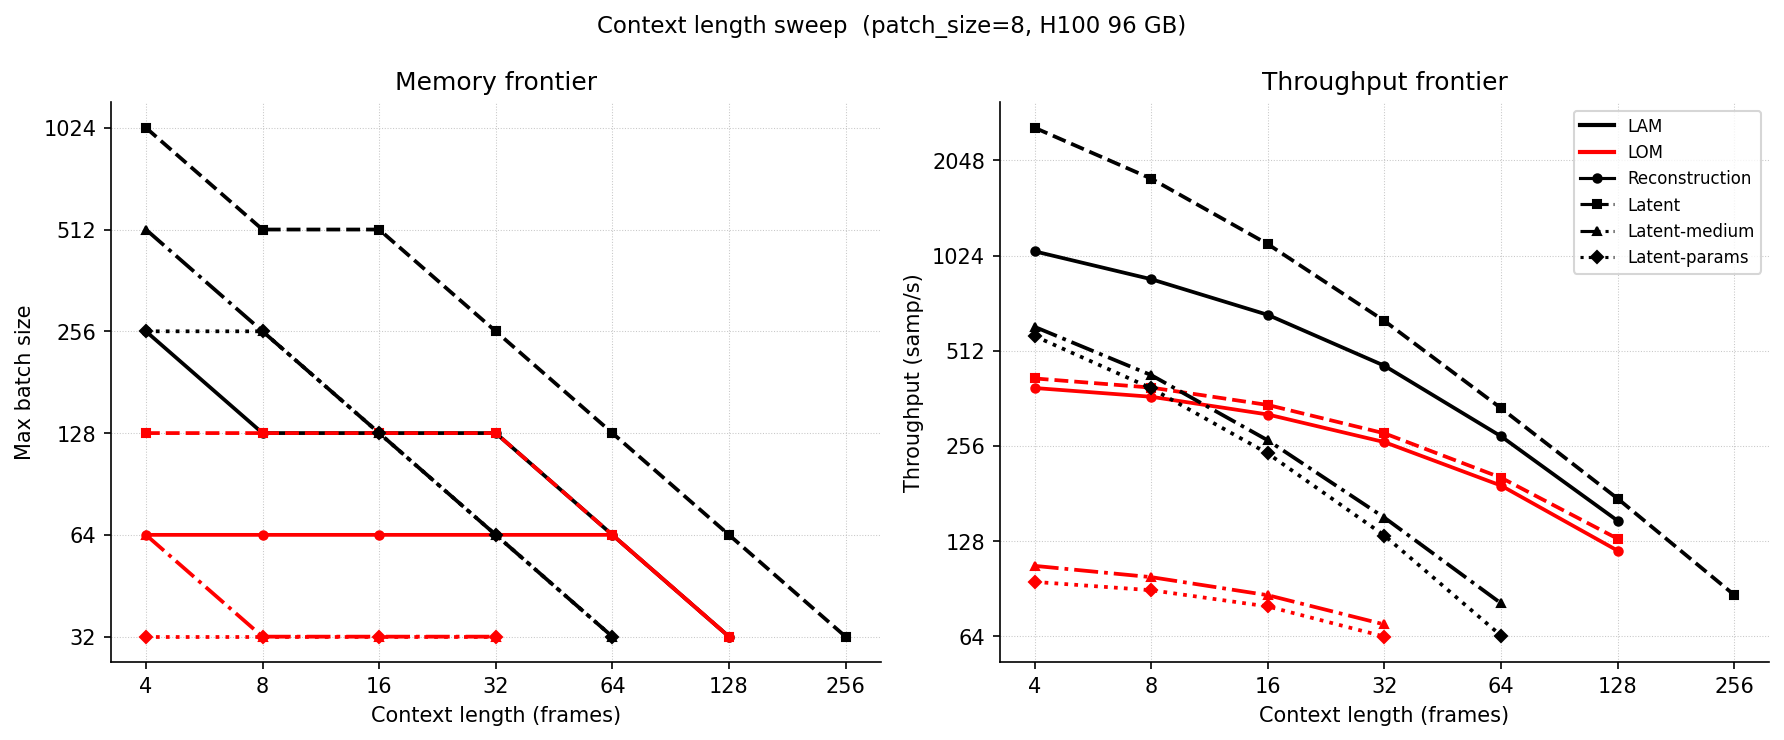
\includegraphics[width=\linewidth]{figures/context_length}
\caption{Context-length Pareto frontier on an 96\,GB GPU.
Black lines = LAM (horizon=1); red lines = LOM (horizon=128).
Line style encodes architecture: solid = Reconstruction, dashed = Latent,
dash-dot = Latent-medium, dotted = Latent-params.
\emph{Left}: largest fitting batch size per context length.
\emph{Right}: throughput (samples/s) at that batch size.}
\label{fig:context_length}
\end{figure}

\begin{table}[h]
\centering
\caption{LAM pareto results (\texttt{patch\_size=8}, compiled, 96\,GB GPU).
Max batch = largest batch size that fits in memory; samp/s at that batch.
``---'' = OOM at batch$=32$.}
\label{tab:pareto_lam}
\setlength{\tabcolsep}{4pt}
\begin{tabular}{r rr rr rr rr}
\toprule
 & \multicolumn{2}{c}{Reconstruction (311\,M)} & \multicolumn{2}{c}{Latent} & \multicolumn{2}{c}{Latent-medium (288\,M)} & \multicolumn{2}{c}{Latent-params (314\,M)} \\
\cmidrule(lr){2-3}\cmidrule(lr){4-5}\cmidrule(lr){6-7}\cmidrule(lr){8-9}
ctx & max b & samp/s & max b & samp/s & max b & samp/s & max b & samp/s \\
\midrule
  4 & $\ge$256 & 1264 & 2048 & 3547 & 1024 &  897 & 256 &  547 \\
  8 & $\ge$256 & 1053 & 1024 & 2231 &  512 &  562 & 256 &  381 \\
 16 & $\ge$256 &  796 &  512 & 1276 &  256 &  322 & 128 &  217 \\
 32 &  128 &  527 &  256 &  667 &  128 &  168 &  64 &  116 \\
 64 &  128 &  250 &  128 &  346 &   64 &   88 &  32 &   58 \\
128 &   64 &  167 &   64 &  178 &   32 &   45 & --- &  --- \\
256 &   32 &   86 &   32 &   88 &  --- &  --- & --- &  --- \\
\bottomrule
\end{tabular}
\end{table}

JEPA-compute matches STT's context reach (ctx$=256$ at batch$=32$) while
sustaining 3--4$\times$ higher throughput at short contexts: the pixel
reconstruction head in STT carries the same backbone compute but adds a
large logits tensor ($B \times H{\times}W \times \text{vocab}$) that caps
the fitting batch size.  JEPA-params, despite matching STT in total parameter
count, exhausts memory earlier because its 12-layer backbone accumulates
proportionally more activation memory; its DynamicsModel head is negligible.
This makes JEPA-compute the most memory-efficient choice for long-context
training, and JEPA-medium the natural candidate when additional backbone
capacity is warranted without the overhead of pixel reconstruction.

Tables~\ref{tab:pareto_lom} and~\ref{tab:horizon_lom} summarise the numerical results.

\begin{table}[h]
\centering
\caption{LOM context pareto (\texttt{patch\_size=8}, horizon=128, compiled, 96\,GB GPU).
``---'' = OOM at batch$=32$.}
\label{tab:pareto_lom}
\setlength{\tabcolsep}{5pt}
\begin{tabular}{r rr rr rr}
\toprule
 & \multicolumn{2}{c}{Reconstruction-LOM (311\,M)} & \multicolumn{2}{c}{Latent-LOM} & \multicolumn{2}{c}{Latent-medium-LOM (288\,M)} \\
\cmidrule(lr){2-3}\cmidrule(lr){4-5}\cmidrule(lr){6-7}
ctx & max b & samp/s & max b & samp/s & max b & samp/s \\
\midrule
  4 &  64 & 220 &  64 & 155 &  32 &  41 \\
  8 &  64 & 204 &  64 & 150 &  32 &  39 \\
 16 &  64 & 183 &  64 & 137 &  32 &  35 \\
 32 &  64 & 148 &  64 & 116 & --- & --- \\
 64 &  32 & 103 &  64 &  91 & --- & --- \\
128 &  32 &  66 &  32 &  60 & --- & --- \\
\bottomrule
\end{tabular}
\end{table}

\begin{figure}[h]
\centering
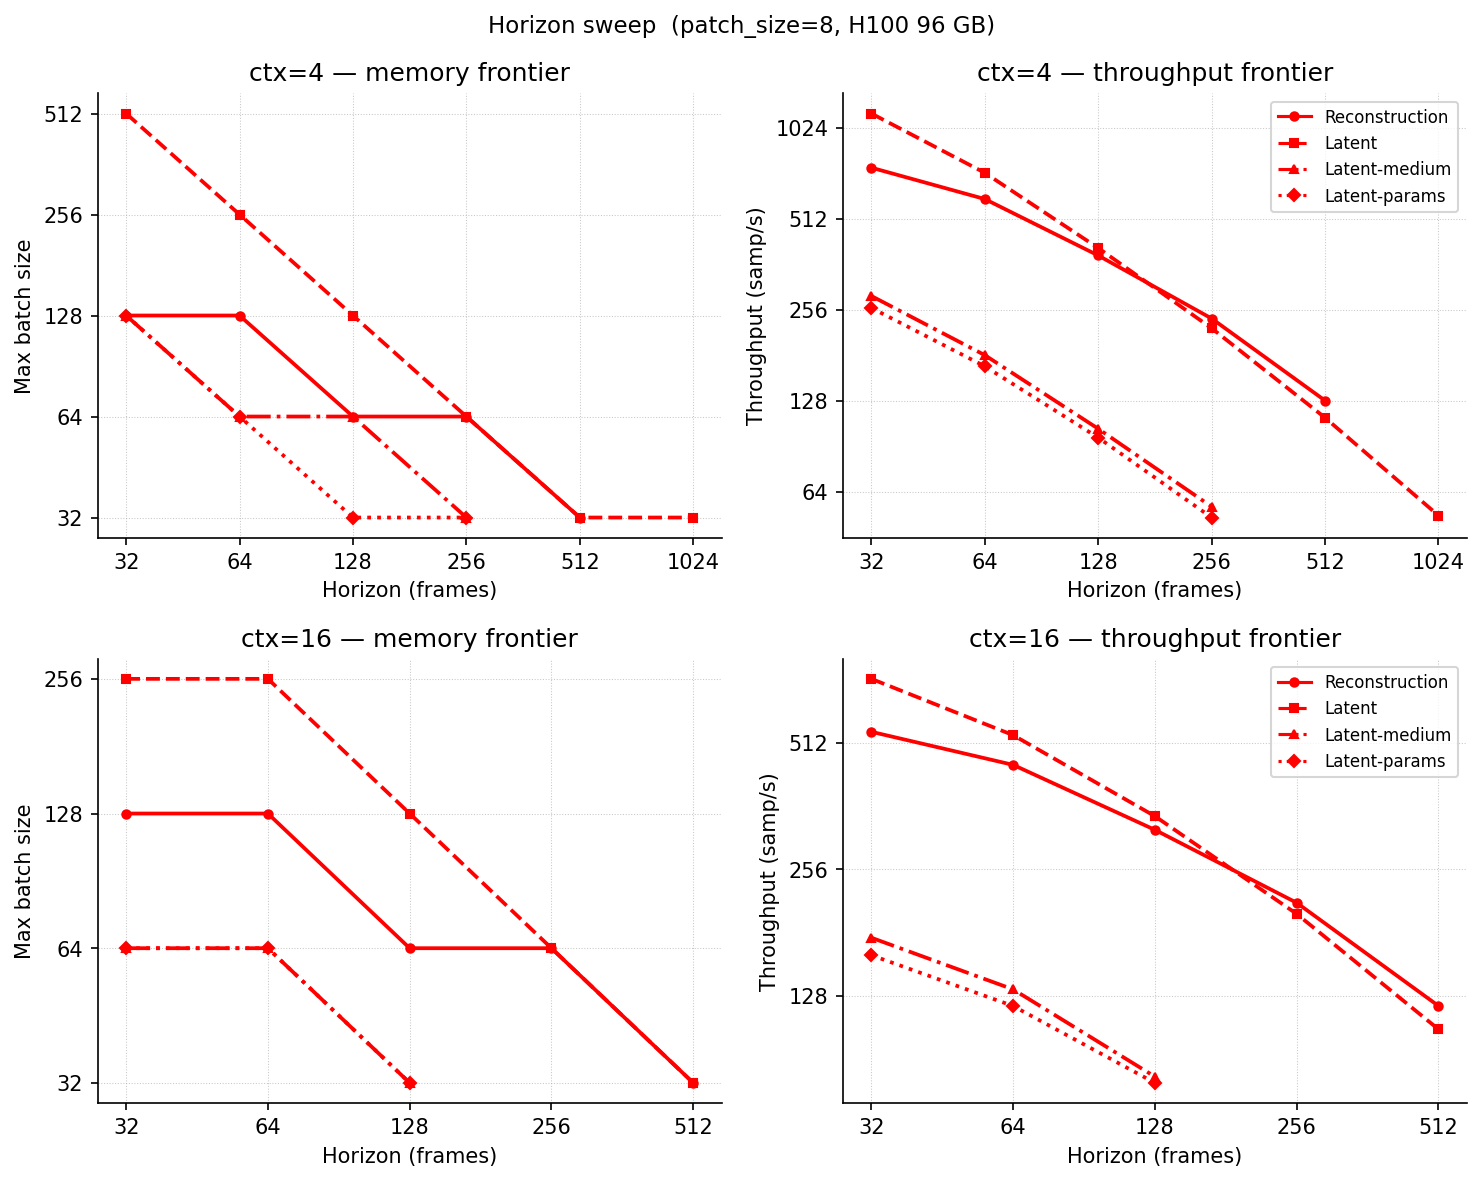
\includegraphics[width=\linewidth]{figures/horizon}
\caption{LOM horizon sweep at fixed ctx=4.
Line style encodes architecture: solid = Reconstruction, dashed = Latent,
dash-dot = Latent-medium, dotted = Latent-params.
\emph{Left}: largest fitting batch size per horizon.
\emph{Right}: throughput (samples/s) at that batch size.}
\label{fig:horizon_lom}
\end{figure}

\begin{table}[h]
\centering
\caption{Maximum affordable horizon (batch$\ge 32$) at fixed ctx=4.
``---'' = OOM at batch$=32$ even for the shortest horizon tested.}
\label{tab:horizon_lom}
\setlength{\tabcolsep}{6pt}
\begin{tabular}{r rrr}
\toprule
horizon & Reconstruction-LOM & Latent-LOM & Latent-medium-LOM \\
\midrule
  4 & 512 & 256 & 128 \\
 32 & 512 & 256 &  64 \\
 64 & 512 & 256 &  32 \\
\bottomrule
\end{tabular}
\end{table}

The Reconstruction encoder is dominated by its two pixel dynamics heads (268\,M of 311\,M total),
which cap the fitting batch size early but are memory-independent of horizon length.
The Latent variants carry negligible dynamics heads but pay for EMA target encoders that must
process the full horizon sequence, limiting maximum horizon more than Reconstruction at equivalent
context.  Latent-params-LOM exhausts the 96\,GB budget at every context length and is not a
viable training configuration at this scale.

\newpage
% \newpage
\section*{NeurIPS Paper Checklist}

%%% BEGIN INSTRUCTIONS %%%
% The checklist is designed to encourage best practices for responsible machine learning research, addressing issues of reproducibility, transparency, research ethics, and societal impact. Do not remove the checklist: {\bf The papers not including the checklist will be desk rejected.} The checklist should follow the references and follow the (optional) supplemental material.  The checklist does NOT count towards the page
% limit. 

% Please read the checklist guidelines carefully for information on how to answer these questions. For each question in the checklist:
% \begin{itemize}
%     \item You should answer \answerYes{}, \answerNo{}, or \answerNA{}.
%     \item \answerNA{} means either that the question is Not Applicable for that particular paper or the relevant information is Not Available.
%     \item Please provide a short (1–2 sentence) justification right after your answer (even for NA). 
%    % \item {\bf The papers not including the checklist will be desk rejected.}
% \end{itemize}

% {\bf The checklist answers are an integral part of your paper submission.} They are visible to the reviewers, area chairs, senior area chairs, and ethics reviewers. You will be asked to also include it (after eventual revisions) with the final version of your paper, and its final version will be published with the paper.

% The reviewers of your paper will be asked to use the checklist as one of the factors in their evaluation. While "\answerYes{}" is generally preferable to "\answerNo{}", it is perfectly acceptable to answer "\answerNo{}" provided a proper justification is given (e.g., "error bars are not reported because it would be too computationally expensive" or "we were unable to find the license for the dataset we used"). In general, answering "\answerNo{}" or "\answerNA{}" is not grounds for rejection. While the questions are phrased in a binary way, we acknowledge that the true answer is often more nuanced, so please just use your best judgment and write a justification to elaborate. All supporting evidence can appear either in the main paper or the supplemental material, provided in appendix. If you answer \answerYes{} to a question, in the justification please point to the section(s) where related material for the question can be found.

% IMPORTANT, please:
% \begin{itemize}
%     \item {\bf Delete this instruction block, but keep the section heading ``NeurIPS Paper Checklist"},
%     \item  {\bf Keep the checklist subsection headings, questions/answers and guidelines below.}
%     \item {\bf Do not modify the questions and only use the provided macros for your answers}.
% \end{itemize} 
 

%%% END INSTRUCTIONS %%%


\begin{enumerate}

\item {\bf Claims}
    \item[] Question: Do the main claims made in the abstract and introduction accurately reflect the paper's contributions and scope?
    \item[] Answer: \answerYes{} % Replace by \answerYes{}, \answerNo{}, or \answerNA{}.
    \item[] Justification: The abstract claims that: (i) NAVIX is a direct drop-in JAX re-implementation of MiniGrid, and (ii) it achieves $>160\,000{\times}$ simulated-step throughput in batch mode and supports $2\,048$ agents on one A100 80 GB. Section~\ref{sec:experiments:speed} reports a $4.4\times 10^{1}$ average speedup across environments without accounting for the increased throughput. Section~\ref{sec:experiments:throughput} demonstrates by batching the computation also across multiple agents, up to $2\,048$, NAVIX can achieve a $>160\,000{\times}$ speedup compared to the MiniGrid version, which is instead limited in scalability by its CPU-based architecture.
    \item[] Guidelines:
    \begin{itemize}
        \item The answer NA means that the abstract and introduction do not include the claims made in the paper.
        \item The abstract and/or introduction should clearly state the claims made, including the contributions made in the paper and important assumptions and limitations. A No or NA answer to this question will not be perceived well by the reviewers. 
        \item The claims made should match theoretical and experimental results, and reflect how much the results can be expected to generalize to other settings. 
        \item It is fine to include aspirational goals as motivation as long as it is clear that these goals are not attained by the paper. 
    \end{itemize}

\item {\bf Limitations}
    \item[] Question: Does the paper discuss the limitations of the work performed by the authors?
    \item[] Answer: \answerYes{} % Replace by \answerYes{}, \answerNo{}, or \answerNA{}.
    \item[] Justification: We remark here the dependence on modern GPUs, i.e., NVidia A100 80GB or better, to reproduce the results. Furthermore, NAVIX is limited by the omission of a few MiniGrid variants that cannot be immediately jittable. Both limitations are stated in Section~\ref{sec:conclusions}.
    \item[] Guidelines:
    \begin{itemize}
        \item The answer NA means that the paper has no limitation while the answer No means that the paper has limitations, but those are not discussed in the paper. 
        \item The authors are encouraged to create a separate "Limitations" section in their paper.
        \item The paper should point out any strong assumptions and how robust the results are to violations of these assumptions (e.g., independence assumptions, noiseless settings, model well-specification, asymptotic approximations only holding locally). The authors should reflect on how these assumptions might be violated in practice and what the implications would be.
        \item The authors should reflect on the scope of the claims made, e.g., if the approach was only tested on a few datasets or with a few runs. In general, empirical results often depend on implicit assumptions, which should be articulated.
        \item The authors should reflect on the factors that influence the performance of the approach. For example, a facial recognition algorithm may perform poorly when image resolution is low or images are taken in low lighting. Or a speech-to-text system might not be used reliably to provide closed captions for online lectures because it fails to handle technical jargon.
        \item The authors should discuss the computational efficiency of the proposed algorithms and how they scale with dataset size.
        \item If applicable, the authors should discuss possible limitations of their approach to address problems of privacy and fairness.
        \item While the authors might fear that complete honesty about limitations might be used by reviewers as grounds for rejection, a worse outcome might be that reviewers discover limitations that aren't acknowledged in the paper. The authors should use their best judgment and recognize that individual actions in favor of transparency play an important role in developing norms that preserve the integrity of the community. Reviewers will be specifically instructed to not penalize honesty concerning limitations.
    \end{itemize}

\item {\bf Theory assumptions and proofs}
    \item[] Question: For each theoretical result, does the paper provide the full set of assumptions and a complete (and correct) proof?
    \item[] Answer: \answerNA{} % Replace by \answerYes{}, \answerNo{}, or \answerNA{}.
    \item[] Justification: The paper does not include theoretical results.
    \item[] Guidelines:
    \begin{itemize}
        \item The answer NA means that the paper does not include theoretical results. 
        \item All the theorems, formulas, and proofs in the paper should be numbered and cross-referenced.
        \item All assumptions should be clearly stated or referenced in the statement of any theorems.
        \item The proofs can either appear in the main paper or the supplemental material, but if they appear in the supplemental material, the authors are encouraged to provide a short proof sketch to provide intuition. 
        \item Inversely, any informal proof provided in the core of the paper should be complemented by formal proofs provided in appendix or supplemental material.
        \item Theorems and Lemmas that the proof relies upon should be properly referenced. 
    \end{itemize}

    \item {\bf Experimental result reproducibility}
    \item[] Question: Does the paper fully disclose all the information needed to reproduce the main experimental results of the paper to the extent that it affects the main claims and/or conclusions of the paper (regardless of whether the code and data are provided or not)?
    \item[] Answer: \answerYes{} % Replace by \answerYes{}, \answerNo{}, or \answerNA{}.
    \item[] Justification: Instructions on how to reproduce all experiments can be found in Section~\ref{sec:experiments}. Hyperparameters for the baselines can be found as described in Appendix~\ref{app:hyperparameters} and in the config files at \repourl/tree/speedup/baselines/rejax/configs.
    \item[] Guidelines:
    \begin{itemize}
        \item The answer NA means that the paper does not include experiments.
        \item If the paper includes experiments, a No answer to this question will not be perceived well by the reviewers: Making the paper reproducible is important, regardless of whether the code and data are provided or not.
        \item If the contribution is a dataset and/or model, the authors should describe the steps taken to make their results reproducible or verifiable. 
        \item Depending on the contribution, reproducibility can be accomplished in various ways. For example, if the contribution is a novel architecture, describing the architecture fully might suffice, or if the contribution is a specific model and empirical evaluation, it may be necessary to either make it possible for others to replicate the model with the same dataset, or provide access to the model. In general. releasing code and data is often one good way to accomplish this, but reproducibility can also be provided via detailed instructions for how to replicate the results, access to a hosted model (e.g., in the case of a large language model), releasing of a model checkpoint, or other means that are appropriate to the research performed.
        \item While NeurIPS does not require releasing code, the conference does require all submissions to provide some reasonable avenue for reproducibility, which may depend on the nature of the contribution. For example
        \begin{enumerate}
            \item If the contribution is primarily a new algorithm, the paper should make it clear how to reproduce that algorithm.
            \item If the contribution is primarily a new model architecture, the paper should describe the architecture clearly and fully.
            \item If the contribution is a new model (e.g., a large language model), then there should either be a way to access this model for reproducing the results or a way to reproduce the model (e.g., with an open-source dataset or instructions for how to construct the dataset).
            \item We recognize that reproducibility may be tricky in some cases, in which case authors are welcome to describe the particular way they provide for reproducibility. In the case of closed-source models, it may be that access to the model is limited in some way (e.g., to registered users), but it should be possible for other researchers to have some path to reproducing or verifying the results.
        \end{enumerate}
    \end{itemize}


\item {\bf Open access to data and code}
    \item[] Question: Does the paper provide open access to the data and code, with sufficient instructions to faithfully reproduce the main experimental results, as described in supplemental material?
    \item[] Answer: \answerYes{} % Replace by \answerYes{}, \answerNo{}, or \answerNA{}.
    \item[] Justification: The full NAVIX code is avilable at \repourl. Documentation is available at \onlinedocs. The folder \repourl/tree/speedup/benchmarks contains the code to run the experiments in Section~\ref{sec:experiments:speed}~and~\ref{sec:experiments:throughput}. The code to reproduce the baselines is available at \repourl/tree/speedup/baselines/rejax.
    \item[] Guidelines:
    \begin{itemize}
        \item The answer NA means that paper does not include experiments requiring code.
        \item Please see the NeurIPS code and data submission guidelines (\url{https://nips.cc/public/guides/CodeSubmissionPolicy}) for more details.
        \item While we encourage the release of code and data, we understand that this might not be possible, so “No” is an acceptable answer. Papers cannot be rejected simply for not including code, unless this is central to the contribution (e.g., for a new open-source benchmark).
        \item The instructions should contain the exact command and environment needed to run to reproduce the results. See the NeurIPS code and data submission guidelines (\url{https://nips.cc/public/guides/CodeSubmissionPolicy}) for more details.
        \item The authors should provide instructions on data access and preparation, including how to access the raw data, preprocessed data, intermediate data, and generated data, etc.
        \item The authors should provide scripts to reproduce all experimental results for the new proposed method and baselines. If only a subset of experiments are reproducible, they should state which ones are omitted from the script and why.
        \item At submission time, to preserve anonymity, the authors should release anonymized versions (if applicable).
        \item Providing as much information as possible in supplemental material (appended to the paper) is recommended, but including URLs to data and code is permitted.
    \end{itemize}


\item {\bf Experimental setting/details}
    \item[] Question: Does the paper specify all the training and test details (e.g., data splits, hyperparameters, how they were chosen, type of optimizer, etc.) necessary to understand the results?
    \item[] Answer: \answerYes{} % Replace by \answerYes{}, \answerNo{}, or \answerNA{}.
    \item[] Justification: Details on hyperparameters and training configurations can be found as described in Appendix~\ref{app:hyperparameters} and at \repourl/tree/speedup/baselines/rejax/configs.
    \item[] Guidelines:
    \begin{itemize}
        \item The answer NA means that the paper does not include experiments.
        \item The experimental setting should be presented in the core of the paper to a level of detail that is necessary to appreciate the results and make sense of them.
        \item The full details can be provided either with the code, in appendix, or as supplemental material.
    \end{itemize}

\item {\bf Experiment statistical significance}
    \item[] Question: Does the paper report error bars suitably and correctly defined or other appropriate information about the statistical significance of the experiments?
    \item[] Answer: \answerYes{} % Replace by \answerYes{}, \answerNo{}, or \answerNA{}.
    \item[] Justification: Results are accompanied by error bars, and their meaning is reported in the correspondig sections. In particular, shaded areas in Figure~\ref{fig:baselines} show $5$-$95$ percentile confidence intervals, as described in Section~\ref{sec:experiments:baselines}. Error bars in Figures~\ref{fig:speedup-envs},~\ref{fig:speedup-steps},~\ref{fig:throughput-envs},~and\ref{fig:throughput-ppo} represent standard errors as described in Section~\ref{sec:experiments:speed}.
    \item[] Guidelines:
    \begin{itemize}
        \item The answer NA means that the paper does not include experiments.
        \item The authors should answer "Yes" if the results are accompanied by error bars, confidence intervals, or statistical significance tests, at least for the experiments that support the main claims of the paper.
        \item The factors of variability that the error bars are capturing should be clearly stated (for example, train/test split, initialization, random drawing of some parameter, or overall run with given experimental conditions).
        \item The method for calculating the error bars should be explained (closed form formula, call to a library function, bootstrap, etc.)
        \item The assumptions made should be given (e.g., Normally distributed errors).
        \item It should be clear whether the error bar is the standard deviation or the standard error of the mean.
        \item It is OK to report 1-sigma error bars, but one should state it. The authors should preferably report a 2-sigma error bar than state that they have a 96\% CI, if the hypothesis of Normality of errors is not verified.
        \item For asymmetric distributions, the authors should be careful not to show in tables or figures symmetric error bars that would yield results that are out of range (e.g. negative error rates).
        \item If error bars are reported in tables or plots, The authors should explain in the text how they were calculated and reference the corresponding figures or tables in the text.
    \end{itemize}

\item {\bf Experiments compute resources}
    \item[] Question: For each experiment, does the paper provide sufficient information on the computer resources (type of compute workers, memory, time of execution) needed to reproduce the experiments?
    \item[] Answer: \answerYes{} % Replace by \answerYes{}, \answerNo{}, or \answerNA{}.
    \item[] Justification: All experiments are run on a single Nvidia A100 80Gb, and Intel(R) Xeon(R) Silver 4310 CPU @ 2.10GHz and 128Gb of RAM., as stated in Section~\ref{sec:experiments}.
    \item[] Guidelines:
    \begin{itemize}
        \item The answer NA means that the paper does not include experiments.
        \item The paper should indicate the type of compute workers CPU or GPU, internal cluster, or cloud provider, including relevant memory and storage.
        \item The paper should provide the amount of compute required for each of the individual experimental runs as well as estimate the total compute. 
        \item The paper should disclose whether the full research project required more compute than the experiments reported in the paper (e.g., preliminary or failed experiments that didn't make it into the paper). 
    \end{itemize}
    
\item {\bf Code of ethics}
    \item[] Question: Does the research conducted in the paper conform, in every respect, with the NeurIPS Code of Ethics \url{https://neurips.cc/public/EthicsGuidelines}?
    \item[] Answer: \answerYes{} % Replace by \answerYes{}, \answerNo{}, or \answerNA{}.
    \item[] Justification: 
    \item[] Guidelines:
    \begin{itemize}
        \item The answer NA means that the authors have not reviewed the NeurIPS Code of Ethics.
        \item If the authors answer No, they should explain the special circumstances that require a deviation from the Code of Ethics.
        \item The authors should make sure to preserve anonymity (e.g., if there is a special consideration due to laws or regulations in their jurisdiction).
    \end{itemize}


\item {\bf Broader impacts}
    \item[] Question: Does the paper discuss both potential positive societal impacts and negative societal impacts of the work performed?
    \item[] Answer: \answerYes{} % Replace by \answerYes{}, \answerNo{}, or \answerNA{}.
    \item[] Justification: Section~\ref{sec:broader-impact} analyses the broader impacts of NAVIX, including the positive effects of democratizing RL research, lowering energy use—and and the negative possibilities such as enabling faster development of malicious autonomous agents. 
    \item[] Guidelines:
    \begin{itemize}
        \item The answer NA means that there is no societal impact of the work performed.
        \item If the authors answer NA or No, they should explain why their work has no societal impact or why the paper does not address societal impact.
        \item Examples of negative societal impacts include potential malicious or unintended uses (e.g., disinformation, generating fake profiles, surveillance), fairness considerations (e.g., deployment of technologies that could make decisions that unfairly impact specific groups), privacy considerations, and security considerations.
        \item The conference expects that many papers will be foundational research and not tied to particular applications, let alone deployments. However, if there is a direct path to any negative applications, the authors should point it out. For example, it is legitimate to point out that an improvement in the quality of generative models could be used to generate deepfakes for disinformation. On the other hand, it is not needed to point out that a generic algorithm for optimizing neural networks could enable people to train models that generate Deepfakes faster.
        \item The authors should consider possible harms that could arise when the technology is being used as intended and functioning correctly, harms that could arise when the technology is being used as intended but gives incorrect results, and harms following from (intentional or unintentional) misuse of the technology.
        \item If there are negative societal impacts, the authors could also discuss possible mitigation strategies (e.g., gated release of models, providing defenses in addition to attacks, mechanisms for monitoring misuse, mechanisms to monitor how a system learns from feedback over time, improving the efficiency and accessibility of ML).
    \end{itemize}
    
\item {\bf Safeguards}
    \item[] Question: Does the paper describe safeguards that have been put in place for responsible release of data or models that have a high risk for misuse (e.g., pretrained language models, image generators, or scraped datasets)?
    \item[] Answer: \answerNA{} % Replace by \answerYes{}, \answerNo{}, or \answerNA{}.
    \item[] Justification: NAVIX releases only an environment library, not a pretrained model or large scraped dataset. The code confers no novel dual-use capability beyond the long-established MiniGrid baseline, so additional safeguards are unnecessary.
    \item[] Guidelines:
    \begin{itemize}
        \item The answer NA means that the paper poses no such risks.
        \item Released models that have a high risk for misuse or dual-use should be released with necessary safeguards to allow for controlled use of the model, for example by requiring that users adhere to usage guidelines or restrictions to access the model or implementing safety filters. 
        \item Datasets that have been scraped from the Internet could pose safety risks. The authors should describe how they avoided releasing unsafe images.
        \item We recognize that providing effective safeguards is challenging, and many papers do not require this, but we encourage authors to take this into account and make a best faith effort.
    \end{itemize}

\item {\bf Licenses for existing assets}
    \item[] Question: Are the creators or original owners of assets (e.g., code, data, models), used in the paper, properly credited and are the license and terms of use explicitly mentioned and properly respected?
    \item[] Answer: \answerYes{} % Replace by \answerYes{}, \answerNo{}, or \answerNA{}.
    \item[] Justification: NAVIX is released under Apache 2.0, as stated on the main repository \repourl/blob/main/LICENSE, with the license file and copyright header included in the repository. MiniGrid is released under MIT license, as stated in the corresponding repo \url{https://github.com/Farama-Foundation/Minigrid/blob/master/LICENSE}. JAX is released under Apache 2.0 as stated in the corresponding repository \url{https://github.com/jax-ml/jax/blob/main/LICENSE}.
    \item[] Guidelines:
    \begin{itemize}
        \item The answer NA means that the paper does not use existing assets.
        \item The authors should cite the original paper that produced the code package or dataset.
        \item The authors should state which version of the asset is used and, if possible, include a URL.
        \item The name of the license (e.g., CC-BY 4.0) should be included for each asset.
        \item For scraped data from a particular source (e.g., website), the copyright and terms of service of that source should be provided.
        \item If assets are released, the license, copyright information, and terms of use in the package should be provided. For popular datasets, \url{paperswithcode.com/datasets} has curated licenses for some datasets. Their licensing guide can help determine the license of a dataset.
        \item For existing datasets that are re-packaged, both the original license and the license of the derived asset (if it has changed) should be provided.
        \item If this information is not available online, the authors are encouraged to reach out to the asset's creators.
    \end{itemize}

\item {\bf New assets}
    \item[] Question: Are new assets introduced in the paper well documented and is the documentation provided alongside the assets?
    \item[] Answer: \answerYes{} % Replace by \answerYes{}, \answerNo{}, or \answerNA{}.
    \item[] Justification: Footnote 1 links to the public GitHub repository: \repourl. Code is everywhere documented, and API docs and installation instructtions are available at \onlinedocs.
    \item[] Guidelines:
    \begin{itemize}
        \item The answer NA means that the paper does not release new assets.
        \item Researchers should communicate the details of the dataset/code/model as part of their submissions via structured templates. This includes details about training, license, limitations, etc. 
        \item The paper should discuss whether and how consent was obtained from people whose asset is used.
        \item At submission time, remember to anonymize your assets (if applicable). You can either create an anonymized URL or include an anonymized zip file.
    \end{itemize}

\item {\bf Crowdsourcing and research with human subjects}
    \item[] Question: For crowdsourcing experiments and research with human subjects, does the paper include the full text of instructions given to participants and screenshots, if applicable, as well as details about compensation (if any)? 
    \item[] Answer: \answerNA{} % Replace by \answerYes{}, \answerNo{}, or \answerNA{}.
    \item[] Justification: No human-subject or crowd-sourcing studies were conducted.
    \item[] Guidelines:
    \begin{itemize}
        \item The answer NA means that the paper does not involve crowdsourcing nor research with human subjects.
        \item Including this information in the supplemental material is fine, but if the main contribution of the paper involves human subjects, then as much detail as possible should be included in the main paper. 
        \item According to the NeurIPS Code of Ethics, workers involved in data collection, curation, or other labor should be paid at least the minimum wage in the country of the data collector. 
    \end{itemize}

\item {\bf Institutional review board (IRB) approvals or equivalent for research with human subjects}
    \item[] Question: Does the paper describe potential risks incurred by study participants, whether such risks were disclosed to the subjects, and whether Institutional Review Board (IRB) approvals (or an equivalent approval/review based on the requirements of your country or institution) were obtained?
    \item[] Answer: \answerNA{} % Replace by \answerYes{}, \answerNo{}, or \answerNA{}.
    \item[] Justification: Not applicable—no human-subject research was performed.
    \item[] Guidelines:
    \begin{itemize}
        \item The answer NA means that the paper does not involve crowdsourcing nor research with human subjects.
        \item Depending on the country in which research is conducted, IRB approval (or equivalent) may be required for any human subjects research. If you obtained IRB approval, you should clearly state this in the paper. 
        \item We recognize that the procedures for this may vary significantly between institutions and locations, and we expect authors to adhere to the NeurIPS Code of Ethics and the guidelines for their institution. 
        \item For initial submissions, do not include any information that would break anonymity (if applicable), such as the institution conducting the review.
    \end{itemize}

\item {\bf Declaration of LLM usage}
    \item[] Question: Does the paper describe the usage of LLMs if it is an important, original, or non-standard component of the core methods in this research? Note that if the LLM is used only for writing, editing, or formatting purposes and does not impact the core methodology, scientific rigorousness, or originality of the research, declaration is not required.
    %this research? 
    \item[] Answer: \answerNA{} % Replace by \answerYes{}, \answerNo{}, or \answerNA{}.
    \item[] Justification: 
    \item[] Guidelines:
    \begin{itemize}
        \item The answer NA means that the core method development in this research does not involve LLMs as any important, original, or non-standard components.
        \item Please refer to our LLM policy (\url{https://neurips.cc/Conferences/2025/LLM}) for what should or should not be described.
    \end{itemize}

\end{enumerate}
\end{document}
